% Diagram of Android activity life cycle
% Author: Pavel Seda 
\documentclass[border=10pt]{standalone}
%%%<
\usepackage{verbatim}
%%%>
\usepackage{pgf, tikz}
\usetikzlibrary{arrows, automata}
\usepackage{amssymb}
\usetikzlibrary{arrows.meta}
\tikzset{%
  >={Latex[width=2mm,length=2mm]},
  % Specifications for style of nodes:
            base/.style = {rectangle, rounded corners, draw=black,
                           minimum height=1cm,
                           text width=3cm,
                           font=\sffamily},
      definition/.style = {base, fill=green!30},
       theorem/.style = {base, fill=red!30, text width=3cm},
}
\begin{document}    



% Drawing part, node distance is 1.5 cm and every node
% is prefilled with white background
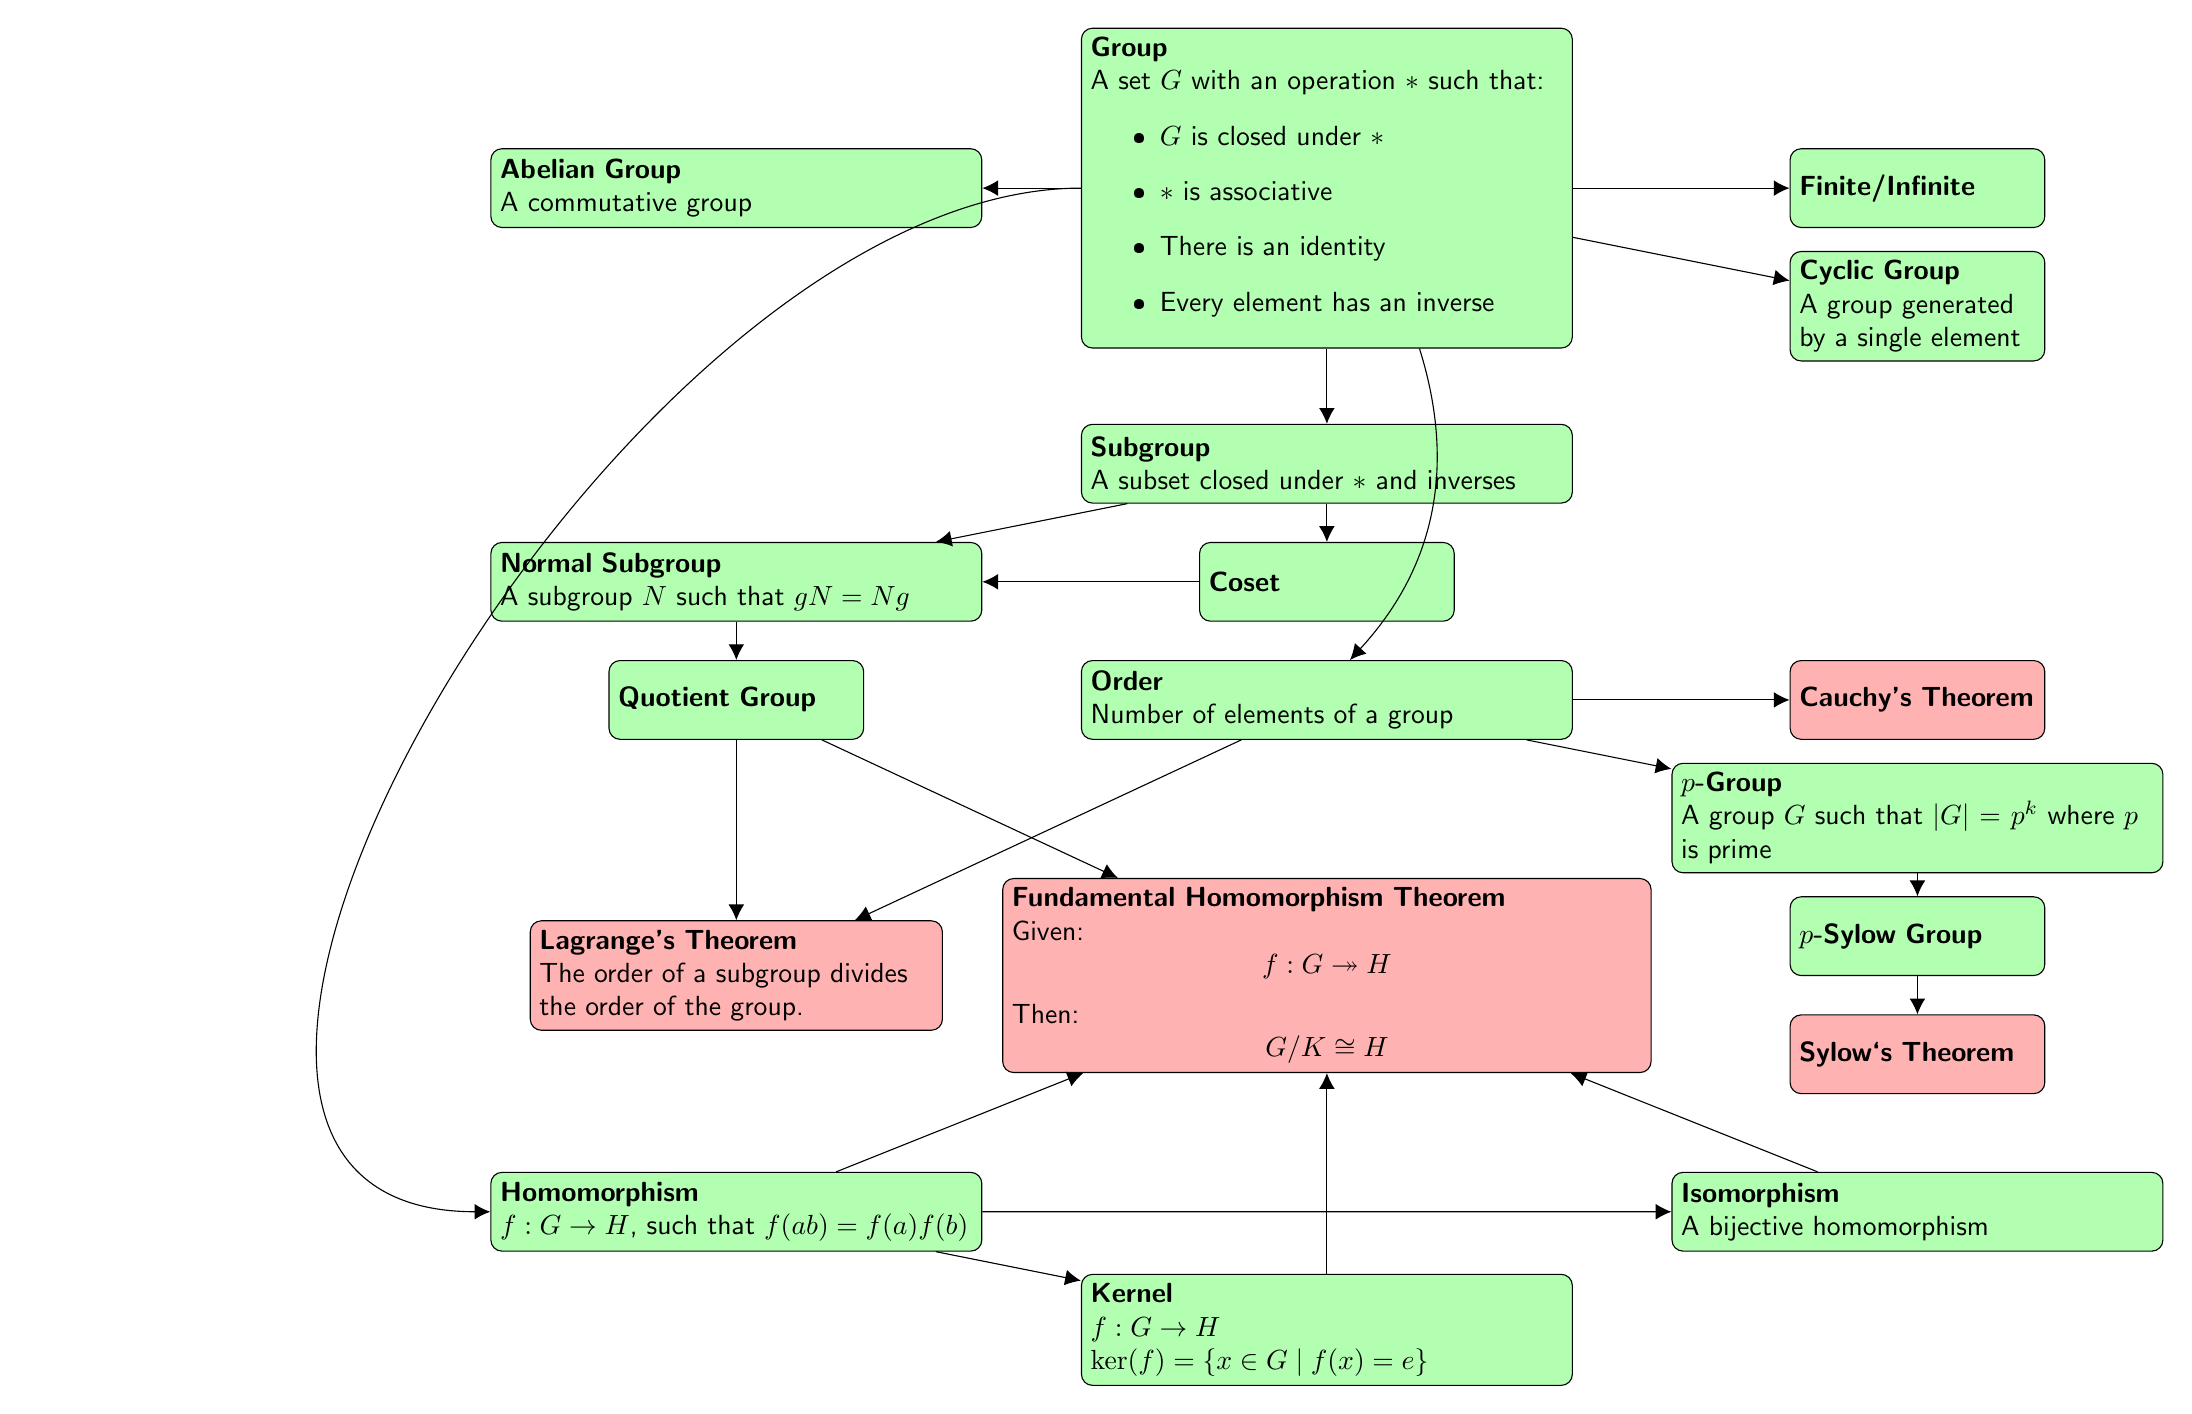
\begin{tikzpicture}[
  ->,
    node distance=1.5cm,
    every node/.style={fill=white, font=\sffamily}, 
    align=left,
    auto]

  \node(group)              [definition, text width=6cm]                              {\vbox {\textbf{Group}\newline
                                                                    A set $G$ with an operation $\ast$ such that:
                                                                {\begin{itemize}
                                                                    \item $G$ is closed under $\ast$
                                                                    \item $\ast$ is associative
                                                                    \item There is an identity
                                                                    \item Every element has an inverse
                                                                \end{itemize}}}};

  \node(abelianGroup)      [definition, left of=group, xshift=-6cm, text width=6cm]  {\textbf{Abelian Group}\newline
                                                                    A commutative group};

  \node(finite)            [definition, right of=group, xshift=6cm]   {\textbf{Finite/Infinite}};

  \node(cyclic)            [definition, below of=finite]                        {\textbf{Cyclic Group}\newline A group generated by a single element};

  \node(subgroup)            [definition, below of=group, text width=6cm, yshift=-2cm]   {\textbf{Subgroup}\newline
                                                                         A subset closed under $\ast$ and inverses};

  \node(coset)            [definition, below of=subgroup]   {\textbf{Coset}};
  \node(normal)            [definition, left of=coset, xshift=-6cm, text width=6cm]   {\textbf{Normal Subgroup}\newline A subgroup $N$ such that $gN = Ng$};
  \node(quotient)            [definition, below of=normal]   {\textbf{Quotient Group}};
  \node(order)            [definition, right of=quotient, xshift=6cm, text width=6cm]   {\textbf{Order}\newline Number of elements of a group};
  \node(cauchy)            [theorem, right of=order, xshift=6cm]   {\textbf{Cauchy's Theorem}};
  \node(pGroup)            [definition, below of=cauchy, text width=6cm]   {\textbf{$p$-Group}\newline A group $G$ such that $|G| = p^k$ where $p$ is prime};
  \node(pSylow)            [definition, below of=pGroup]   {\textbf{$p$-Sylow Group}};
  \node(sylow)            [theorem, below of=pSylow]   {\textbf{Sylow`s Theorem}};
  \node(lagrange)            [theorem, below of=quotient, text width=5cm, yshift=-2cm]   {\textbf{Lagrange's Theorem}\newline The order of a subgroup divides the order of the group.};
  
  \node(homomorphism)            [definition, below of=quotient, text width=6cm, yshift=-5cm]   {\textbf{Homomorphism}\newline
                                                                                                $f: G \rightarrow H$, such that $f(ab) = f(a)f(b)$};


  \node(isomorphism)            [definition, below of=sylow, text width=6cm, yshift=-0.5cm]   {\textbf{Isomorphism}\newline
                                                                                                A bijective homomorphism};

  \node(fht)            [theorem, left of=sylow, text width=8cm, xshift=-6cm, yshift=1cm]   {\textbf{Fundamental Homomorphism Theorem}\newline
                                                                                    Given:
                                                                                    $$f: G \twoheadrightarrow H$$
                                                                                    Then:
                                                                                    $$G/K\cong H$$};
  
  \node(kernel)            [definition, below of=fht, text width=6cm, yshift=-3cm]   {\textbf{Kernel}\newline
                                                                                    $f: G \rightarrow H$\\
                                                                                    $\ker(f) = \{x \in G \mid f(x) = e\}$};
  
% \path (cauchy) edge [bend right] node {} (group);
                  

  % Specification of lines between nodes specified above
  % with aditional nodes for description 
  \draw[->]             (group) -- (abelianGroup);
  \draw[->]             (group) -- (finite);
  \draw[->]             (group) -- (subgroup);
  \draw[->]             (subgroup) -- (coset);
  \draw[->]             (subgroup) -- (normal);
  \draw[->]             (coset) -- (normal);
  \draw[->]             (normal) -- (quotient);
  \draw[->]             (group) to[in=180, out=270, bend left] (order);
  \draw[->]             (order) -- (cauchy);
  \draw[->]             (order) -- (pGroup);

  \draw[->]             (quotient) -- (lagrange);
  \draw[->]             (order) -- (lagrange);

  \draw[->]             (homomorphism) -- (isomorphism);
  \draw[->]             (homomorphism) -- (kernel);
  \draw[->]             (homomorphism) -- (fht);
  \draw[->]             (isomorphism) -- (fht);
  \draw[->]             (kernel) -- (fht);
  \draw[->]             (group) to[in=180,out=180] (homomorphism);
  \draw[->]             (quotient) -- (fht);
  \draw[->]             (pGroup) -- (pSylow);
  \draw[->]             (pSylow) -- (sylow);
  \draw[->]             (group) -- (cyclic);
  
\end{tikzpicture}
\end{document}
